\documentclass{beamer}


\usepackage{amssymb,amsmath}
\usepackage{graphicx}
\usepackage{url}
\usepackage{color}
\usepackage{relsize}		% For \smaller
\usepackage{url}			% For \url
\usepackage{epstopdf}	% Included EPS files automatically converted to PDF to include with pdflatex
\usepackage{pagenote}[continuous,page]

%For MindMaps
% \usepackage{tikz}%
% \usetikzlibrary{mindmap,trees,arrows}%

%%% Color Definitions %%%%%%%%%%%%%%%%%%%%%%%%%%%%%%%%%%%%%%%%%%%%%%%%%%%%%%%%%
%\definecolor{bordercol}{RGB}{40,40,40}
%\definecolor{headercol1}{RGB}{186,215,230}
%\definecolor{headercol2}{RGB}{80,80,80}
%\definecolor{headerfontcol}{RGB}{0,0,0}
%\definecolor{boxcolor}{RGB}{186,215,230}

%%% Save space in lists. Use this after the opening of the list %%%%%%%%%%%%%%%%
%\newcommand{\compresslist}{
%	\setlength{\itemsep}{1pt}
%	\setlength{\parskip}{0pt}
%	\setlength{\parsep}{0pt}
%}

%\setbeameroption{show notes on top}

% You should run 'pdflatex' TWICE, because of TOC issues.

% Rename this file.  A common temptation for first-time slide makers
% is to name it something like ``my_talk.tex'' or
% ``john_doe_talk.tex'' or even ``discrete_math_seminar_talk.tex''.
% You really won't like any of these titles the second time you give a
% talk.  Try naming your tex file something more descriptive, like
% ``riemann_hypothesis_short_proof_talk.tex''.  Even better (in case
% you recycle 99% of a talk, but still want to change a little, and
% retain copies of each), how about
% ``riemann_hypothesis_short_proof_MIT-Colloquium.2000-01-01.tex''?

\mode<presentation>
{
  % A tip: pick a theme you like first, and THEN modify the color theme, and then add math content.
  % Warsaw is the theme selected by default in Beamer's installation sample files.

  %%%%%%%%%%%%%%%%%%%%%%%%%%%% THEME
  %\usetheme{Madrid}		% No subsection
  \usetheme{AnnArbor}  % Subsection on top, no color


  %\usetheme{Antibes}
  %\usetheme{Bergen}
  %\usetheme{Berkeley}		% bem bacana - menu esquerdo
  %\usetheme{Berlin}
  %\usetheme{Boadilla}
  %\usetheme{boxes}
  %\usetheme{CambridgeUS}		% bem bacana - menu superior
  %\usetheme{Copenhagen}
  %\usetheme{Darmstadt}
  %\usetheme{default}
  %\usetheme{Dresden}
  %\usetheme{Frankfurt}
  %\usetheme{Goettingen}
  %\usetheme{Hannover}		% bem bacana - menu esquerdo
  %\usetheme{Ilmenau}
  %\usetheme{JuanLesPins}
  %\usetheme{Luebeck}
  %\usetheme{Malmoe}
  %\usetheme{Marburg}		% bem bacana - menu direito
  %\usetheme{Montpellier}
  %\usetheme{PaloAlto}		% bem bacana - menu esquerdo
  %\usetheme{Pittsburgh}
  %\usetheme{Rochester}		%bacana
  %\usetheme{Singapore}
  %\usetheme{Szeged}
  %\usetheme{Warsaw}

  %%%%%%%%%%%%%%%%%%%%%%%%%%%% COLOR THEME
  %\usecolortheme{default}		% branco, azul clarinho
  \usecolortheme{crane}		% Very yellow (ok)

  %\usecolortheme{albatross}		% azul escuro, massa
  %\usecolortheme{beetle}		% cinza, menu azul
  %\usecolortheme{dolphin}		% azul e branco, legal
  %\usecolortheme{dove}			% cinza e branco, feio
  %\usecolortheme{fly}			% todo cinza, horrível
  %\usecolortheme{lily}			% parece o default
  %\usecolortheme{orchid}		% azul e branco, ok
  %\usecolortheme{rose}			% branco e violeta-claro, bonito
  %\usecolortheme{seagull}		% cinza, feio
  %\usecolortheme{seahorse}		% nhé, meio feio
  %\usecolortheme{sidebartab}		% Azul, branco, destaque na tab, interessante
  %\usecolortheme{structure}		% bichado
  %\usecolortheme{whale}		% Azul e branco, bem bonito

  %%%%%%%%%%%%%%%%%%%%%%%%%%%% OUTER THEME
  \useoutertheme{default}
  %\useoutertheme{infolines}
  %\useoutertheme{miniframes}
  %\useoutertheme{shadow}
  %\useoutertheme{sidebar}
  %\useoutertheme{smoothbars}
  %\useoutertheme{smoothtree}
  %\useoutertheme{split}
  %\useoutertheme{tree}

  %%%%%%%%%%%%%%%%%%%%%%%%%%%% INNER THEME
  \useinnertheme{circles}
  %\useinnertheme{default}
  %\useinnertheme{inmargin}
  %\useinnertheme{rectangles}
  %\useinnertheme{rounded}

  %%%%%%%%%%%%%%%%%%%%%%%%%%%%%%%%%%%

  \setbeamercovered{invisible} % or whatever (possibly just delete it)
  % To change behavior of \uncover from graying out to totally
  % invisible, can change \setbeamercovered to invisible instead of
  % transparent. apparently there are also 'dynamic' modes that make
  % the amount of graying depend on how long it'll take until the
  % thing is uncovered.

}


% Get rid of nav bar
\beamertemplatenavigationsymbolsempty

% Use short top
%\usepackage[headheight=12pt,footheight=12pt]{beamerthemeboxes}
%\addheadboxtemplate{\color{black}}{
%\hskip0.5cm
%\color{white}
%\insertshortauthor \ \ \ \
%\insertframenumber \ \ \ \ \ \ \
%\insertsection \ \ \ \ \ \ \ \ \ \ \ \ \ \ \ \ \  \insertsubsection
%\hskip0.5cm}
%\addheadboxtemplate{\color{black}}{
%\color{white}
%\ \ \ \
%\insertsection
%}
%\addheadboxtemplate{\color{black}}{
%\color{white}
%\ \ \ \
%\insertsubsection
%}

% Insert frame number at bottom of the page.
% \usefoottemplate{\hfil\tiny{\color{black!90}\insertframenumber}}

%% makes the ppagenote command for figure references at the end.

\usepackage[english]{babel}
%qq\usepackage[latin1]{inputenc}
\usepackage{CJKutf8}
\usepackage{subfigure}

\usepackage{times}
\usepackage[T1]{fontenc}

\makepagenote
\renewcommand{\notenumintext}[1]{}
\newcommand{\ppagenote}[1]{\pagenote[Page \insertframenumber]{#1}}

\title[Programming Challenges]{GB20602 - Programming Challenges}
\author[Claus Aranha]{Claus Aranha\\{\footnotesize caranha@cs.tsukuba.ac.jp}}
\institute[U. Tsukuba]{University of Tsukuba, Department of Computer Sciences}


\title[]{Programming Challenges}
\subtitle[]{Week 5 - Number Theory and Backtracking}
\author[Claus Aranha]{Claus Aranha\\{\footnotesize caranha\@@cs.tsukuba.ac.jp}}
\institute{College of Information Sciences}
\date{2015-05-18\\{\tiny Last updated \today}}

\begin{document}

\section{Introduction}
\subsection{outline}

\begin{frame}
\maketitle
\end{frame}

\begin{frame}
  \frametitle{No classes next week!}

  No classes on \alert{18/5, 22/5, 25/5}.
  \vfill
  Next class on \structure{29/5}
\end{frame}

\begin{frame}
\frametitle{Outline}
\begin{block}{}
  Today we will see some more classes of algorithms using some of the
  concepts in the previous classes. You might have seen some of these
  before.
\end{block}
\begin{itemize}
\item Number Theoretic Algorithms
  \begin{itemize}
  \item Calculating Prime Numbers
  \item Greatest Common Divisor
  \end{itemize}
\item Backtracking
\end{itemize}
\end{frame}

\section{Primality}
\subsection{Calculating Primes}
\begin{frame}
  \frametitle{Calculating Primes}
\end{frame}

\begin{frame}[singleslide,fragile]
  \frametitle{How do we test whether $n$ is prime?}
  \begin{block}{Naive Algorithm}
    We test the numbers $i$ between 2 and $\sqrt{n}$, to see if 
    $n \text{ mod } i=0$
  \end{block}
  \vfill
\begin{verbatim}
for(i = 2; i < sqrt{n}+1; i++}
  {
    if (n%i == 0)
      return FALSE;
  }
\end{verbatim}
  \vfill
  \begin{block}{}
    What is the problem in the code above?
  \end{block}
\end{frame}

\begin{frame}[singleslide,fragile]
  \frametitle{How do we test whether $n$ is prime? (2)}
\begin{verbatim}
for(i = 2; i < sqrt{n}; i++}
  {
    if (n%i == 0)
      return FALSE;
  }
\end{verbatim}
\vfill
\begin{block}{What is the problem in the code above}
  \begin{itemize}
  \item The square root function can induce imprecisions in the system;
  \item We should use $i*i < n$;
  \item Is there a problem with the use of $i*i$?
  \end{itemize}
\end{block}
\end{frame}

\begin{frame}[singleslide,fragile]
  \frametitle{How do we test whether $n$ is prime? (3)}
\begin{verbatim}
for(i = 2; i*i < n; i++}
  {
    if (n%i == 0)
      return FALSE;
  }
\end{verbatim}
\vfill
\begin{block}{Is there a problem with the use of $i*i$?}
  \begin{itemize}
  \item For big enough $n$, $i*i$ may overflow;
  \item We can calculate $i*i$ without a multiplication, using a \emph{recurrence}
  \item $i^2 = (i-1)^2 + 2(i-1) + 1$
  \item Replace $i$ in the \emph{for} with the recurrence value above;
  \end{itemize}
\end{block}
\end{frame}

\begin{frame}
  \frametitle{Calculating primes in the naive way}
  \begin{itemize}
  \item We used the idea of a \structure{recurrence relation} from
    last class;
  \item The recurrence eliminated multiplication and exponentiation
    operations; (Not only for recursion!)
  \item This kind of thought process is very useful when fine tuning
    algorithms;
  \end{itemize}
\end{frame}

\begin{frame}
  \frametitle{Real-world Primality Testing}
  {\small
  \begin{block}{Fermat's primality testing}
    \begin{itemize}
      \item Most libraries test for primality using an approximated
        test, such as the \structure{Fermat's Primality Test}. 
      \item $n$ is \emph{probably} prime if for a random number $a$:
    \end{itemize}
  \end{block}
  \begin{equation*}
    a^{(n-1)} \equiv 1 ({mod} n)
  \end{equation*}
  \begin{block}{}
    \begin{itemize}
    \item The more $a$'s you try, the higher the probability of
      primality;
    \item There are stronger versions of this test, but the principle
      is the same;
    \end{itemize}
  \end{block}
  }
\end{frame}

\subsection{Greatest Common Divisor}
\begin{frame}
  \frametitle{Calculating the Greatest Common Divisor}
  
  \begin{block}{Greatest Common Divisor (GDC)}
    Given two positive integers, $a$ and $b$, the GDC is the largest
    integer $c$ so that $a\%c = 0$ and $b\%c = 0$
  \end{block}
  \vfill
  \begin{block}{}
    Useful for reducing fractions (two classes ago), and many other
    algorithms.
  \end{block}
  \begin{center}
    Ideas for algorithms? What are their complexities?
  \end{center}
\end{frame}

\begin{frame}
  \frametitle{Algorithms for calculating the GDC}
  \begin{block}{Naive Algorithm}
    \begin{itemize}
    \item Calculate the factorization of $a$
    \item For each factor $f_a$, calculate $b\%f_a$
    \item Should we factor $a$ or $b$? Hard to tell!
    \item What is the complexity of this algorithm?
    \end{itemize}
  \end{block}
\end{frame}
\begin{frame}
  \frametitle{Algorithms for calculating the GDC}
  \begin{block}{Euclid's Algorithm}
    \begin{itemize}
    \item if $a = bt$, $GCD(a,b) = b$
    \item if $a = bt+r$, $GCD(a,b) = GCD(bt+r,b) = GCD(b,r)$
    \item $GCD(a,b) = GCD(b,a\%b)$ Should we factor $a$ or $b$? Hard to tell!
    \item What is the complexity of this algorithm? -- O(Factorization(a))
    \end{itemize}
  \end{block}
\end{frame}

\begin{frame}
  \frametitle{Why is GCD(a,b) = GCD(b,a\%b)?}
  \begin{columns}[c]
    \column{0.7\textwidth}
    {\small
    \begin{enumerate}
    \item Imagine a rectangle with sides $a$ and $b$;
    \item The \emph{GCD} is the side of largest square that can fill
      this rectangle;
    \item By subtracting $b$ from $a$, we have a new rectangle with
      sides $b$, $a\%b$;
    \item Can you see that a square that would fit the rectangle
      $b,a\%b$, will also fit the rectangle $b,b$?
    \item Consequently, it will also fit the rectangle $a,b$;
    \end{enumerate}
    }
    \column{0.3\textwidth}
    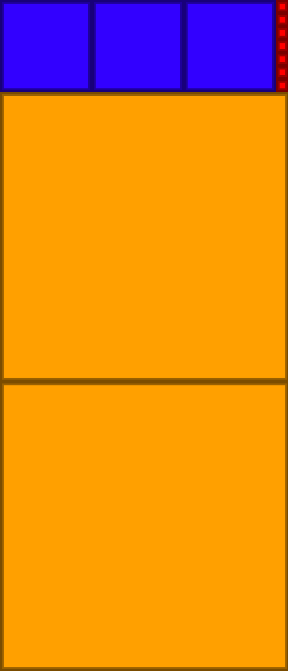
\includegraphics[width=1\textwidth]{img/euclid}
  \end{columns}
\end{frame}

\subsection{For more info}
\begin{frame}
  \frametitle{To know more cool facts about numbers}
  \begin{block}{}
    \begin{itemize}
    \item Proving Concepts using Geometry;
    \item Interesting facts about prime numbers;
    \item $1 + 2 + 3 + 4 + ... = \frac{-1}{12}$
    \end{itemize}
  \end{block}
  \begin{itemize}
  \item Numberphile channel:
  \item \url{https://www.youtube.com/channel/UCoxcjq-8xIDTYp3uz647V5A}
  \end{itemize}  
\end{frame}

\section{Backtracking}
\subsection{Introduction}

% Informal definition
\begin{frame}
  \frametitle{Backtracking}

  \begin{block}{What does the word \emph{Backtracking} means?}
    \emph{To go back on your own steps; To return the same way that
    you came;}
  \end{block}
  \bigskip

  Basic Ideas:
  \begin{itemize}
  \item Try to ``assemble'' a solution;
  \item Return, or ``undo'' some steps if you reach a dead end;
  \item Avoid dead ends as soon as possible (``pruning'');
  \end{itemize}
\end{frame}

% Formal definition
\begin{frame}
  \frametitle{Backtracking -- some important points}
  \begin{block}{Backtracking Algorithm}
    Backtracking is a \structure{systematic method} to iterate through
    \structure{all the possible solutions} of a problem.
  \end{block}
  \bigskip

  \begin{itemize}
  \item Represent the solution as a vector $a = (a_1, a_2, ..., a_n)$;
  \item Each $a_i$ is a step of the solution, taken from a finite set $S_i$\\
    \begin{itemize}
    \item Solution is a set, and $a_i$ is a boolean denoting the presence of $i$;
    \item Solution is a permutation, and $a_i$ is the $i_{th}$ element of the permutation;
    \end{itemize}
  \item This general technique that must be customized for each application;
  \end{itemize}
  \vfill
\end{frame}

\begin{frame}
  \frametitle{Backtracking}
  \begin{block}{Backtracking Algorithm}
    Backtracking is a \structure{systematic method} to iterate through
    \structure{all the possible solutions} of a problem.
  \end{block}
  \begin{enumerate}
  \item At each step in the algorith, start from a partial solution
    ($a_1, a_2, ..., a_k$), and try to extend it, by adding $a_{k+1}$.
  \item After adding a new element, test to see if $a$ is a valid solution.
  \item Test to see if $a$ can be extended again. If so, repeat \structure{(1)}.
  \item If it cannot, remove $a_{k+1}$ and repeat \structure{(1)} with
    another value for $a_{k+1}$.
  \end{enumerate}
  \vfill
\end{frame}

\subsection{Example}

\begin{frame}
  \frametitle{Example: The 8-queen Problem}
  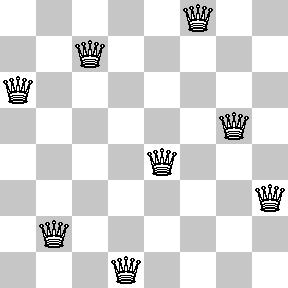
\includegraphics[width=2.5cm]{img/eightqueen}
  \begin{block}{}
    \begin{itemize}
    \item Put $n$ queens in an $n$ by $n$ square board;
    \item No 2 queens can be on the same line, row or diagonal;
    \end{itemize}
  \end{block}
\end{frame}


\begin{frame}
  \frametitle{The n-queen Problem (2)}
  \begin{block}{Thinking about the problem}
    \begin{itemize}
    \item Main question: How do we represent one solution?
      \begin{itemize}
      \item Array of true/false?
      \item Array of x,y position of queens?
      \item Column Representation?
      \end{itemize}
    \end{itemize}
  \end{block}
  \begin{block}{}
    Important question: How many solutions exist for each
    representation?
  \end{block}
\end{frame}

\begin{frame}
  \frametitle{The n-queen Problem (3)}
  \begin{block}{Secondary question: How to search for the solution?}
    \begin{itemize}
    \item Sequential search through all possibilities;
    \item Can we skip some branches that we \structure{KNOW} are dead ends?\\
      {\small(this is called ``pruning'')}
    \end{itemize}
  \end{block}
\end{frame}

\subsection{More on Backtracking}
%% NP Completeness
\begin{frame}
  \frametitle{When should we use Backtracking?}
  \begin{block}{}
    \begin{itemize}
    \item Backtracking is powerful, but very \structure{expensive};
    \item It potentially explores all possible solution patterns;
    \bigskip

    \item We usually want to use backtracking when \structure{an
      efficient solution is not known};
    \item Or when we don't know if an optimal solution exists;
    \bigskip
    \end{itemize}
  \end{block}
\end{frame}

\begin{frame}
  \frametitle{Backtracking Videos}
  \begin{itemize}
  \item Sudoku: \url{http://www.youtube.com/watch?v=pd9awN2xBqw}
  \item Maze: \url{http://www.youtube.com/watch?v=anZlAmtaV1s}
  \item 8-queens: \url{http://www.youtube.com/watch?v=ckC2hFdLff0}
  \end{itemize}
\end{frame}

\begin{frame}
  \frametitle{Backtracking Structure}
  
  \begin{block}{}
    A backtracking algorithm usually includes these three functions:
  \end{block}
  
  \begin{itemize}
    \item \structure{is\_a\_solution(a,k,input);}\\ 
      Tests whether the first $k$ elements of $a$ are a complete
      solution to the problem
      \medskip
    \item \structure{construct\_candidates(a,k,input,c,\&ncandidates);}\\
      Fills the array $c$ with the complete list of possible
      candidates for position $k$;
      \medskip
    \item \structure{process\_solution(a,k,input);}\\
      Prints/counts/etc a complete solution;
  \end{itemize}
\end{frame}


\begin{frame}
  \frametitle{Constructing All Subsets}
  %% TODO: Write some code here
  \begin{itemize}
  \item We can construct all the subsets of $n$ items by iterating on
    all possible $2^n$ vectors of true/false values.
  \item How do we define a solution for ``any subset''?
  \item How do we define a solution for ``any subset with $k$ items''?
  \end{itemize}
\end{frame}

\begin{frame}
  \frametitle{Constructing All Permutations}
  %% TODO: Add some code
  \begin{itemize}
  \item To avoid repeating elements, we need to keep track of what
    elements were already used.
  \item We test whether an element was already used when adding a new
    item to a partial solution.
  \end{itemize}
\end{frame}

\begin{frame}
  \frametitle{Backtracking Looks a bit like DFS...}
  %% TODO: Drawings/improvements

  \begin{itemize}
  \item Backtracking is a generalization of Depth First Search (DFS)
  \item DFS applies to \structure{tree-graphs}, while backtracking
    applies to any data structure;
  \item The graph is built implicitely as the search is performed --
    the entire graph is not necessary to perform the search;
  \end{itemize}
\end{frame}

\begin{frame}
  \frametitle{The Limits of Backtracking}
  \begin{itemize}
  \item Backtracking is an \structure{exhaustive search}; depending on
    the size of the problem, it can take a LONG time.
  \item How to calculate the size of the problem? Remember our class
    on \structure{Combinatorics}.
    \begin{itemize}
    \item How big is a subset problem?
    \item How big is a permutation problem?
    \end{itemize}
  \end{itemize}
\end{frame}

\begin{frame}
  \frametitle{Pruning}
  %TODO: Improve this

  \begin{block}{Pruning}
    Problem specific ``Tricks'' to reduce the number of solutions we
    have to search for.
  \end{block}

  \begin{itemize}
  \item Stopping after the first solution;
  \item Changing the representation;
  \item Checking for invalid/unpromising answers;
  \item etc;
  \end{itemize}
\end{frame}

\section{This Week's Problems}
\subsection{This Week's Problems}
\begin{frame}
  \frametitle{This Week's Problems}
  \begin{itemize}
    \item Light, more Light (Number Theory)
    \item Marbles (Number Theory)
    \item Queue (Recursion)
    \item Tug of War (Recursion)
  \end{itemize}
\end{frame}
\end{document}
